% =====================================================================================================
% Draft: Sections 12.5-12.8 and the abstract's accuracy sentences, rerun under protocol v3.1.
%
% How to merge into paper/main.tex
%   1. Abstract: replace the text from "The accuracy results so far use an earlier single-release
%      mechanism." up to and including the \tocheck{The accuracy numbers in this abstract ...} by the
%      block between BEGIN-ABSTRACT and END-ABSTRACT below. The sentences before it ("In a simulation of
%      the release and solve steps ...") and after it ("End-to-end runs of a full OpenFHE ...") stay.
%   2. Section 12: replace the four subsections "Coefficient accuracy against intersection size (earlier
%      mechanism)", "Does the bias correction matter? (earlier mechanism)", "Benchmark against AdaSSP
%      (earlier mechanism)" and "Intersection size on real data (earlier mechanism)", including their
%      figures, tables and \tocheck items, by the block between BEGIN-SECTIONS and END-SECTIONS.
%      The section labels sec:eval:sim, sec:eval:bias, sec:eval:adassp and sec:eval:sweep are kept, so the
%      references to them elsewhere in the paper still resolve. Every figure and table label is new
%      (suffix _v31) and does not clash with an existing label.
%   3. Text elsewhere that quotes the old numbers and should change with this merge (not edited here):
%      the opening paragraph of Section 12 (it says Sections 12.4-12.9 use the earlier mechanism);
%      Section 10.6, "the mechanism bias is at most 0.75% of the mean squared error"; and in Section 12.9,
%      "The gap to AdaSSP is the noise level, not the ridge rule" (under v3.1 the gap is the ridge rule,
%      see Section 12.7 below) and the oracle-ridge numbers quoted there.
%
% Scripts: experiments/v31_eval/; results: reports/v31_eval/ (README.md, key_numbers.md); figures:
% paper/figures/*_v31.png.
% =====================================================================================================

% ---------------------------------------------------------------- BEGIN-ABSTRACT
In a simulation of the v3.1 release and solve steps at $\delta = 10^{-9}$ on a synthetic population, the stage-1 ridge switches off between $1.0$ and $1.2$ times the intersection size that the protocol parameters predict ($6.0$k to $81$k matched records for $\varepsilon = 8$ to $0.5$). The coefficient error then reaches twice that of non-private least squares at $7.3$k, $23$k and $79$k matched records for $\varepsilon = 8$, $4$ and $2$, and prediction comes within $10\%$ of non-private test error $1.7$--$5.2$ times sooner. On real data with each party normalizing its own block of every row, prediction comes within $10\%$ of non-private test error at $10$k and $5.2$k matched records on protein for $\varepsilon = 1$ and $2$, but not within the $12$k--$14$k records available on bike and pol for $\varepsilon \le 4$. With the same preprocessing, AdaSSP on the joined table has lower test error than v3.1 on $20$ of $29$ datasets at $\varepsilon = 1$, $\delta = 10^{-6}$, because the v3.1 ridge, sized for valid intervals, is a median four to six times larger.
% ---------------------------------------------------------------- END-ABSTRACT

% ---------------------------------------------------------------- BEGIN-SECTIONS
\subsection{Coefficient accuracy against intersection size}
\label{sec:eval:sim}

\paragraph{Setup.} The population has $d_{R} = 4$ and $d_{O} = 6$ features on realistic raw scales (a score, a binary indicator, lognormal income and assets, a count and an age), Toeplitz-correlated with coefficient $0.3$. They are standardized with public population constants and clipped to the population's $99.5\%$ bounds ($B_{R} = 5.59$ with the intercept, $B_{O} = 6.24$, $B_{y} = 2.89$ at $R^2 = 0.5$). The generating slopes give $R^{2} \in \{0.3, 0.5, 0.9\}$. The weakest direction of the clipped design is $\ell = \lambda_{\min}(\Sigma) = 0.599$, estimated from $4$ million population rows, and $\lambda_{\min}(\bA)/n = 0.656$.

The mechanism is v3.1, simulated in plaintext with the implementation's own calibration and solver: a stage-1 release of $(\triu\bB, \bC)$ with s.d.\ $\sigma_1$, the stage-1 rule of Section~\ref{sec:stats:stage1}, a stage-2 release of every $\Op$-dependent entry with s.d.\ $\sigma_2$, the gate $\hat\vartheta \ge 1$, and the solve, with the bias correction off. The simulated noise is Gaussian in the slot domain with the calibrated s.d. The encrypted implementation's measured noise is $0.996\,\sigma_2$ and $0.976\,\sigma_1$ (Section~\ref{sec:eval:crypto}), and its estimates on protein lie inside the simulated range (Section~\ref{sec:eval:e2e}). A further encrypted check in the ridge-on regime is reported at the end of this subsection.

The evaluation uses these settings, which are not protocol defaults: $\delta = 10^{-9}$, $f_1 = 0.1$, $\vartheta^\star = 2.5$, $\kappa_\Psi = 2$, $\alpha = 0.05$ with $\alpha_L = \alpha_U = \alpha/20$, $\by^\top\by$ in stage~2 (it is free for these bounds), and the flooding parameter $\kappa = 40$ for $\varepsilon \le 2$, $44$ at $\varepsilon = 4$ and $48$ at $\varepsilon = 8$. With $\Delta = 86.2$ and $\Delta_G = 77.2$ this gives $\sigma_1 = 2746$, $1411$, $729$, $380$, $202$ and $\sigma_2 = 1022$, $525$, $271$, $141$, $75$ for $\varepsilon = 0.5$, $1$, $2$, $4$, $8$ (Table~\ref{tab:noff_sim}). For each $n$ from $10^{2}$ to $10^{5}$ we draw 200 cohorts. For each cohort and each $\varepsilon$ we run an independent pair of releases, and we report the RMSE of the slopes against the true coefficients.

\begin{figure}[t]
  \centering
  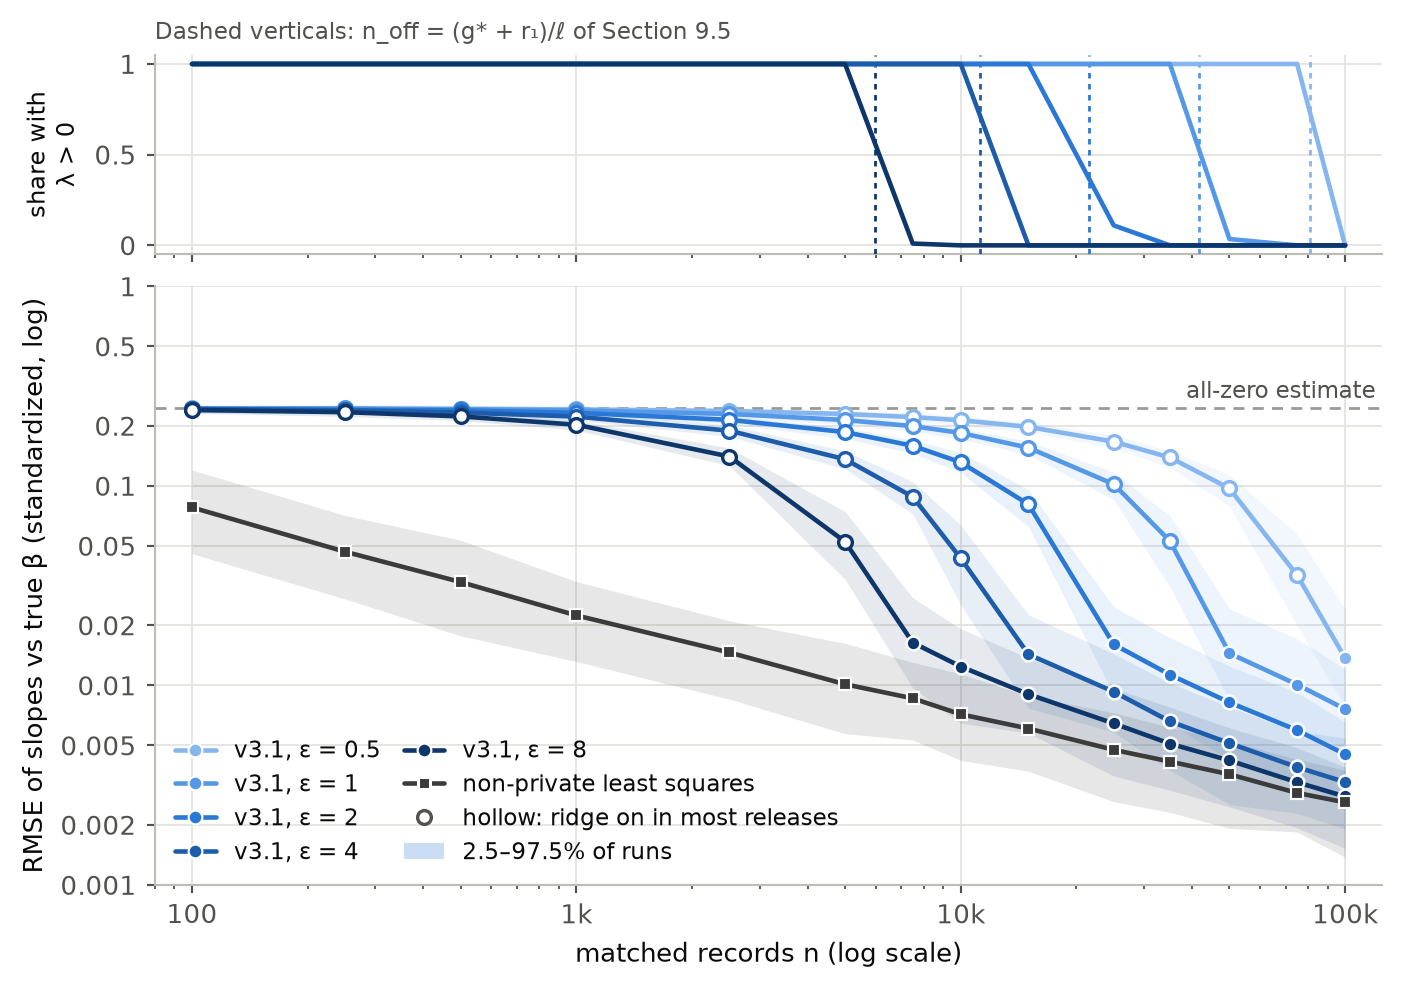
\includegraphics[width=\textwidth]{figures/sim_rmse_vs_n_v31.png}
  \caption{Protocol v3.1, $\delta = 10^{-9}$, $R^2 = 0.5$. Bottom: RMSE of the slopes against the true coefficients (standardized scale) against the intersection size $n$. Lines: median over 200 runs, each with a new cohort and a new pair of releases. Bands: 2.5--97.5\% of runs. Hollow markers: the stage-1 ridge is on in most releases. Grey: non-private least squares on the true matches. Top: share of releases with $\lambda > 0$; dashed verticals at $n_{\mathrm{off}}$ of~\eqref{eq:noff}.}
  \label{fig:sim_rmse_v31}
\end{figure}

\begin{table}[t]
  \centering
  \small
  \caption{Protocol v3.1, $\delta = 10^{-9}$, $R^{2} = 0.5$: median RMSE of the standardized slopes against the true coefficients, with the ratio to the non-private floor in brackets. $^\ast$: the stage-1 ridge is on in most releases.}
  \label{tab:sim_rmse_v31}
  \begin{tabular}{@{}rcccccc@{}}
    \toprule
    $n$ & $\varepsilon = 0.5$ & $\varepsilon = 1$ & $\varepsilon = 2$ & $\varepsilon = 4$ & $\varepsilon = 8$ & OLS floor \\
    \midrule
    $10^{3}$ & 0.242 (10.8)$^\ast$ & 0.239 (10.7)$^\ast$ & 0.232 (10.4)$^\ast$ & 0.222 (9.9)$^\ast$ & 0.203 (9.0)$^\ast$ & 0.0224 \\
    $10^{4}$ & 0.213 (29.8)$^\ast$ & 0.184 (25.7)$^\ast$ & 0.131 (18.3)$^\ast$ & 0.043 (6.0)$^\ast$ & 0.012 (1.7) & 0.0072 \\
    $10^{5}$ & 0.014 (5.3) & 0.0076 (2.9) & 0.0045 (1.7) & 0.0033 (1.3) & 0.0028 (1.1) & 0.0026 \\
    \bottomrule
  \end{tabular}
\end{table}

\paragraph{Results.} Figure~\ref{fig:sim_rmse_v31} and Table~\ref{tab:sim_rmse_v31} show two regimes.
\begin{itemize}[noitemsep]
  \item \emph{Ridge on.} While the stage-1 ridge is on, the estimate is shrunk towards zero, and its RMSE stays close to that of the all-zero estimate ($0.25$). At $n = 10^{4}$ the median RMSE is $0.213$, $0.184$, $0.131$ and $0.043$ for $\varepsilon = 0.5$ to $4$, which is $6$--$30$ times the floor.
  \item \emph{Ridge off.} Once the ridge switches off, the DP error falls like $1/n$, faster than the sampling error, and merges into the floor. The error reaches twice the floor at $n \approx 7.3$k ($\varepsilon = 8$), $23$k ($\varepsilon = 4$) and $79$k ($\varepsilon = 2$). At $\varepsilon = 1$ and $0.5$ the ratio is still $2.9$ and $5.3$ at $n = 10^{5}$.
\end{itemize}
A stronger signal lowers the floor but not the DP error. At $R^2 = 0.9$ the crossings are at $23$k and $51$k ($\varepsilon = 8$, $4$), and none is reached by $10^5$ for $\varepsilon \le 2$. At $R^2 = 0.3$ they are at $7.0$k, $15$k and $56$k ($\varepsilon = 8$, $4$, $2$).

The earlier single-release mechanism ($\delta = 10^{-5}$, committed eigenvalue bound) reached twice the floor at $3.2$k, $9.4$k and $34$k for $\varepsilon = 8$, $4$ and $2$. Under v3.1 these crossings are $2.3$--$2.5$ times larger, close to the ratio $(\sigma_2/\sigma)^2 = 2.1$--$2.5$ of the noise variances.

\begin{table}[t]
  \centering
  \small
  \caption{Stage-1 rule on the simulation population, $\delta = 10^{-9}$: share of 200 releases with $\lambda = 0$ at $n = m\, n_{\mathrm{off}}$, each on a fresh cohort, and the median $\lambda$ at $0.8\,n_{\mathrm{off}}$ against the linear prediction $g^\star + r_1 - n\ell$ of Section~\ref{sec:stats:noff}.}
  \label{tab:noff_check_v31}
  \begin{tabular}{@{}rrcccccrr@{}}
    \toprule
    & & \multicolumn{5}{c}{share with $\lambda = 0$ at $m =$} & \multicolumn{2}{c}{$\lambda$ at $0.8\,n_{\mathrm{off}}$} \\
    \cmidrule(lr){3-7} \cmidrule(l){8-9}
    $\varepsilon$ & $n_{\mathrm{off}}$ & 0.6 & 0.8 & 1.0 & 1.2 & 1.4 & median & predicted \\
    \midrule
    0.5 & 81{,}208 & 0.00 & 0.00 & 0.03 & 0.99 & 1.00 & 14{,}563 & 9{,}721 \\
    1 & 41{,}729 & 0.00 & 0.00 & 0.04 & 0.97 & 1.00 & 7{,}500 & 4{,}995 \\
    2 & 21{,}557 & 0.00 & 0.00 & 0.04 & 0.98 & 1.00 & 4{,}067 & 2{,}580 \\
    4 & 11{,}241 & 0.00 & 0.00 & 0.04 & 0.95 & 1.00 & 2{,}080 & 1{,}346 \\
    8 & 5{,}967 & 0.00 & 0.00 & 0.05 & 0.94 & 1.00 & 1{,}138 & 714 \\
    \bottomrule
  \end{tabular}
\end{table}

\paragraph{When the ridge switches off.} Section~\ref{sec:stats:noff} predicts the switch-off at $n_{\mathrm{off}} = (g^\star + r_1)/\ell$: $81$k, $42$k, $22$k, $11$k and $6.0$k for $\varepsilon = 0.5$ to $8$. The simulation agrees.
\begin{itemize}[noitemsep]
  \item On the grid of Figure~\ref{fig:sim_rmse_v31}, the ridge is on in every release up to $0.92\,n_{\mathrm{off}}$, and in at most $11\%$ of releases from $1.16\,n_{\mathrm{off}}$.
  \item Table~\ref{tab:noff_check_v31} puts the transition between $n_{\mathrm{off}}$ ($3$--$5\%$ of releases off) and $1.2\,n_{\mathrm{off}}$ ($94$--$99\%$ off), as in Table~\ref{tab:noff_sim}.
  \item Below the threshold the rule chooses $1.5$--$1.6$ times the linear prediction, because $\lambda_{\min}(\hat\bG_1)$ is biased downward.
  \item Near $n_{\mathrm{off}}$ the rule takes the $\Op$-block ridge $\Psi = \PiO$ in about half of the releases with $\lambda > 0$ ($51$--$53\%$ at $n_{\mathrm{off}}$), because $\lambda_{\min}(\bA)/n > \ell$. Below $0.8\,n_{\mathrm{off}}$ it never does.
\end{itemize}

\paragraph{Prediction recovers first.} On a held-out sample of the population, the test MSE comes within $10\%$ of that of non-private least squares at $n \approx 0.71\,n_{\mathrm{off}}$ for every $\varepsilon$ at $R^2 = 0.5$ ($4.2$k to $58$k), while the ridge is still on. It comes within $1\%$ at $1.1$--$1.2\,n_{\mathrm{off}}$. Twice-the-floor accuracy on the coefficients needs $1.7$, $2.9$ and $5.2$ times as many records as prediction within $10\%$, for $\varepsilon = 8$, $4$ and $2$.

\paragraph{Coefficients on different scales.} Raw-scale errors cannot be compared across coefficients, so Figure~\ref{fig:sim_eff_v31} shows the \emph{efficiency ratio} $\mathrm{RMSE}_{\mathrm{DP},j}/\mathrm{SE}_{\mathrm{OLS},j}$. It does not change when $x_j$ or $y$ is rescaled. A ratio $r$ means the release is about as accurate as least squares on $n/r^2$ records. While the ridge is on, the ratio grows with $n$ and is largest for the largest coefficients, which the ridge shrinks most. Once $\lambda = 0$ in every release, the ten slopes' ratios lie within $-20\%$ and $+26\%$ of their median, except at $\varepsilon = 8$ and $n \ge 50$k, where one coefficient reaches $+36\%$. Neither block is consistently harder: the $\Op$-block average is $0.90$--$1.17$ times the $\Rp$-block average.

\begin{figure}[t]
  \centering
  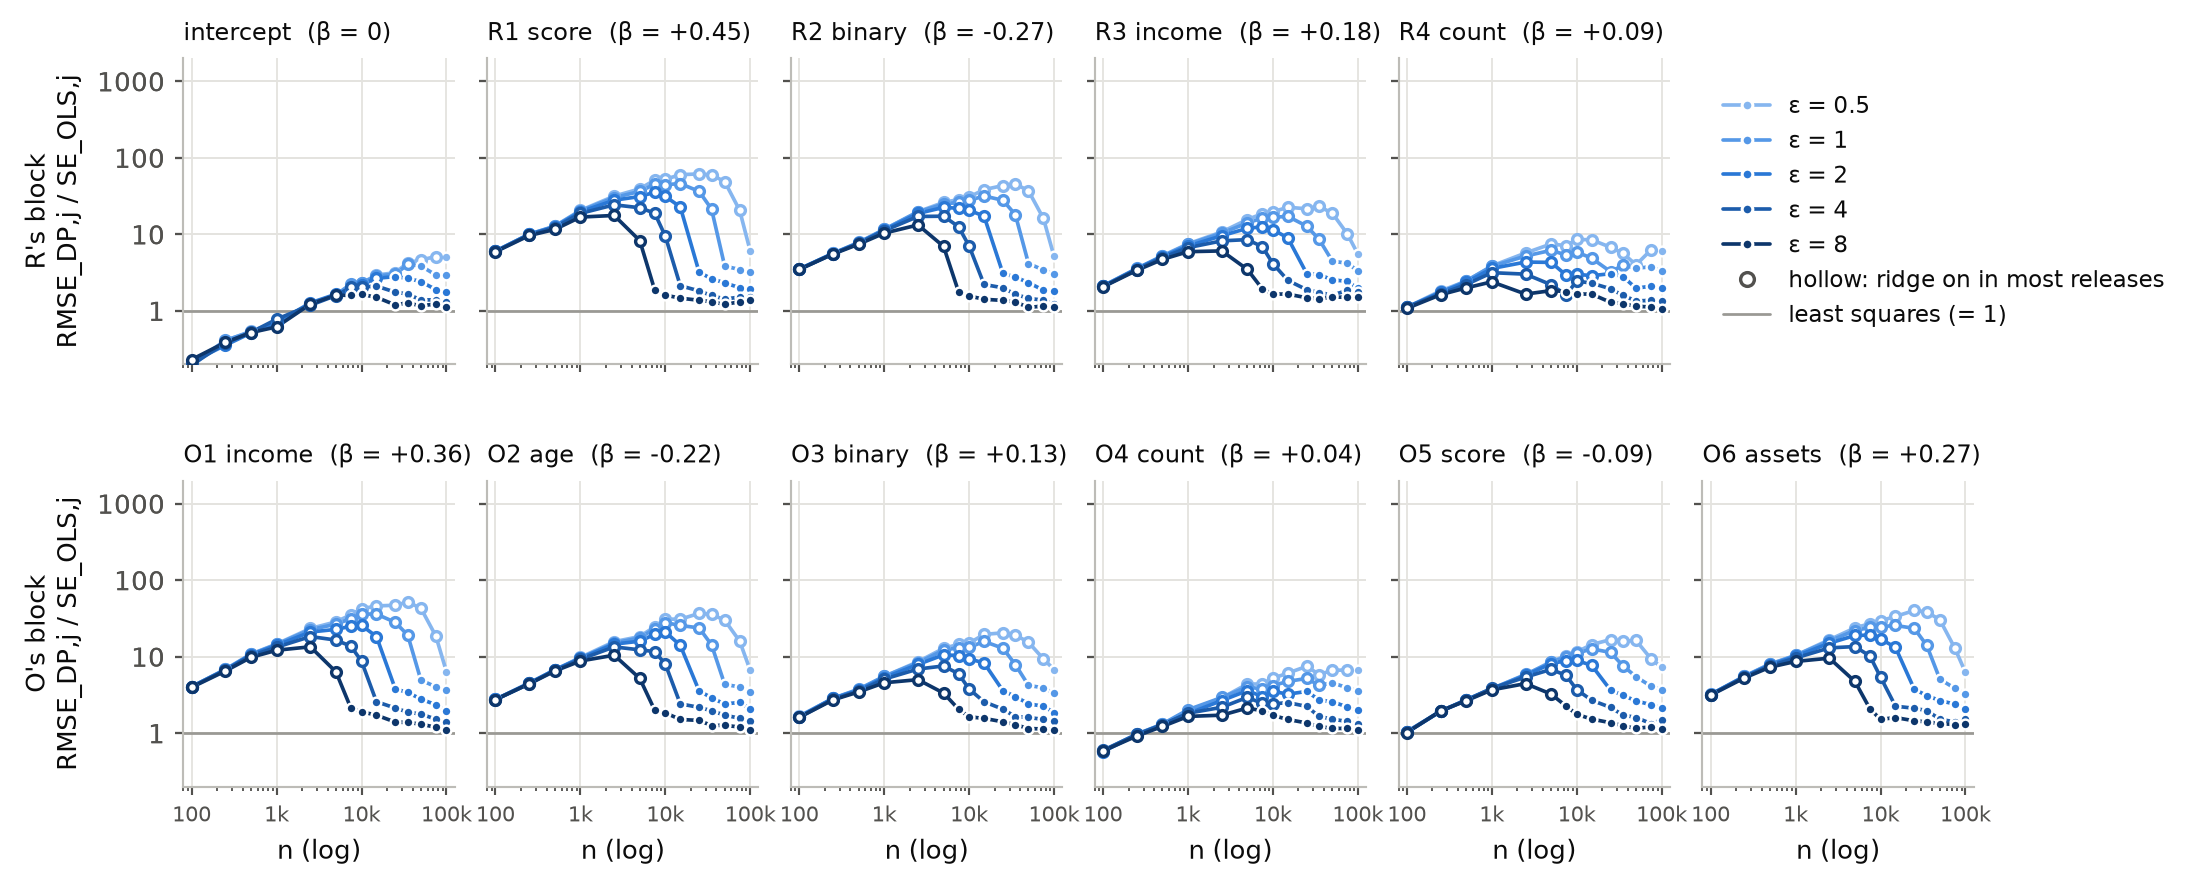
\includegraphics[width=\textwidth]{figures/sim_efficiency_ratio_v31.png}
  \caption{Efficiency ratio $\mathrm{RMSE}_{\mathrm{DP},j}/\mathrm{SE}_{\mathrm{OLS},j}$ per coefficient against $n$, protocol v3.1, $\delta = 10^{-9}$, $R^{2} = 0.5$. Top row: $\Rp$'s block, with the intercept. Bottom row: $\Op$'s block. Hollow markers: the stage-1 ridge is on in most releases.}
  \label{fig:sim_eff_v31}
\end{figure}

\paragraph{Inference.} At $R^2 = 0.5$ every release also runs the intervals of Section~\ref{sec:stats:ci}, with a bootstrap of $2{,}000$ antithetic pairs and no public bound on $\|\bbeta\|$.
\begin{itemize}[noitemsep]
  \item \emph{Wald interval for $\btheta_\lambda$.} It covers $0.945$--$0.965$ of the coefficients in each of the 70 $(n, \varepsilon)$ cells, pooled over the 200 releases and 11 coefficients, with the ridge on or off (target $0.955$).
  \item \emph{Bias-aware interval for $\bbeta$.} When the ridge is off in every release (20 cells), it is finite and covers the true slopes $0.930$--$0.964$ of the time, and the clipped-population coefficients $0.945$--$0.962$; at large $n$ clipping moves the target. While the ridge is on, $\hat L = 0$ in most releases and the interval is unbounded. Where $\hat L > 0$ it is finite but wide: median half-width up to $2.4$, against $0.033$ for the Wald interval.
  \item \emph{Naive reading.} Read as an interval for $\bbeta$, the Wald interval covers only $2$--$60\%$ while the ridge is on.
\end{itemize}
The gate refused no release in any cell, at any $R^2$.

\paragraph{Encrypted check in the ridge-on regime.} We ran the full OpenFHE implementation ten times, in two batches, on one synthetic dataset from this population. It has $n = 10{,}000$ matched records in a register of $12{,}000$ rows padded to $16{,}384$, and we used $\varepsilon = 2$ and $\delta = 10^{-9}$, where the ridge is on ($n_{\mathrm{off}} = 21.6$k). Each run took $29$--$34$\,s.
\begin{itemize}[noitemsep]
  \item The ridge chosen in every run, $8{,}077$--$9{,}296$, lay inside the $95\%$ range of a plaintext simulation of the same mechanism on the same data ($7{,}659$--$10{,}187$).
  \item The Wald interval covered $\btheta_\lambda$ for $105$ of $110$ coefficients.
  \item In the second batch, the decrypted noise on the $306$ stage-1 and $372$ stage-2 entries, standardized by $\sigma_1$ and $\sigma_2$, had s.d.\ $0.98$ and $0.98$, mean $0.02$ and $0.06$, and no value beyond $3.3$; $\bA$ was exact.
  \item Against the simulated distribution of $\tilde\btheta$ given each run's $\lambda$, 109 of the 110 encrypted coefficients lay within $2.5$ s.d. One lay at $3.85$ s.d.; it came from the first batch, whose raw noise was not recorded.
\end{itemize}

\tocheck{Encrypted spot check: one of 110 coefficients deviated by 3.85 s.d. from the simulated distribution (first batch, raw noise not recorded); the second batch's raw noise matches the calibrated s.d. Repeat with about 50 encrypted runs, recording the raw noise, before relying on it.}

% ---------------------------------------------------------------- 12.6
\subsection{Does the bias correction matter?}
\label{sec:eval:bias}

Under v3.1 the ridge comes from stage~1, so it is independent of the stage-2 noise (Proposition~\ref{prop:indep}), and Theorem~\ref{thm:ridge} applies conditionally on $(\lambda, \Psi)$. We ask the question again with the earlier conditional design, at the settings of Section~\ref{sec:eval:sim} ($\delta = 10^{-9}$, $R^2 = 0.5$).
\begin{itemize}[noitemsep]
  \item For each $n \in \{500, 1{,}000, \dots, 128{,}000\}$ (doubling) and each $\varepsilon$ we draw five datasets.
  \item For each dataset we draw four stage-1 releases, each of which fixes $(\lambda, \Psi)$.
  \item For each of these we draw $10{,}000$ antithetic pairs $(\bE, \bff)$, $(-\bE, -\bff)$ of stage-2 releases.
\end{itemize}
The comparison against the true coefficients uses the cohort-level runs of Section~\ref{sec:eval:sim}.

\begin{table}[t]
  \centering
  \small
  \caption{Mechanism bias and the optional correction~\eqref{eq:bc} under v3.1, $\delta = 10^{-9}$, $R^2 = 0.5$; 45 cells ($n$, $\varepsilon$), binned by $\vartheta_0 = \lambda_{\min}(\bG)/(2\sigma_2\sqrt p)$. Bias share and largest standardized bias: maxima over the cells of a bin. MSE ratio: corrected over uncorrected. $K$: smallest number of averaged releases of the same data at which the squared bias equals the variance of the average.}
  \label{tab:bias_v31}
  \setlength{\tabcolsep}{4pt}
  \begin{tabular}{@{}lcccccccr@{}}
    \toprule
    & & & bias$^2$/MSE & $\max_j |b_j|/\mathrm{sd}_j$ & \multicolumn{2}{c}{MSE ratio against} & & \\
    \cmidrule(lr){6-7}
    $\vartheta_0$ & cells & ridge on & (uncorrected) & (uncorrected) & $\btheta_\lambda$ & $\hat\bbeta$ & & $K$ \\
    \midrule
    0--1 & 15 & 15 & 0.001\% & 0.009 & 0.9951--0.9954 & 1.0000--1.0005 & & 81{,}616 \\
    1--2.5 & 6 & 6 & 0.012\% & 0.024 & 0.9952--0.9954 & 1.0009--1.0021 & & 9{,}069 \\
    2.5--7 & 9 & 9 & 0.048\% & 0.044 & 0.9945--0.9952 & 1.0025--1.0109 & & 2{,}118 \\
    7--15 & 5 & 0 & 0.048\% & 0.037 & 0.9960--0.9972 & 0.9960--0.9972 & & 2{,}103 \\
    $\ge 15$ & 10 & 0 & 0.011\% & 0.018 & 0.9990--1.0000 & 0.9990--1.0000 & & 8{,}782 \\
    \bottomrule
  \end{tabular}
\end{table}

No, not even as a variance reduction (Table~\ref{tab:bias_v31}, Figure~\ref{fig:bias_v31}).
\begin{itemize}[noitemsep]
  \item \emph{The bias is negligible.} The mechanism bias of Theorem~\ref{thm:ridge} is at most $0.048\%$ of the mean squared error around $\btheta_\lambda$ in any of the 45 cells. The largest coefficient bias is at most $0.044$ of its standard deviation. The earlier mechanism gave $0.75\%$ and $0.14$. The reason is the stage-1 rule: while the ridge is on it holds $\vartheta_\lambda$ at $7.9$--$9.2$, well above $\vartheta^\star = 2.5$, because of the radius $r_1$; in these cells the ridge is off only from $\vartheta_0 = 9.6$. The bias peaks around the switch-off and decays like $1/\vartheta_0^2$ after it.
  \item \emph{The theorem holds.} Wherever $\vartheta_0 \ge 1$, the simulated bias is $0.997$--$1.010$ times the leading term $\sigma_2^2 M(\bP_\lambda)\btheta_\lambda$.
  \item \emph{Against $\btheta_\lambda$} the correction lowers the mean squared error by at most $0.55\%$: by about $0.5\%$ with the ridge on and by $0.4\%$ or less once it is off. At most $0.05$ percentage points of this come from removing bias; the rest is a variance reduction. The earlier mechanism gave $7$--$12\%$ with the ridge on, when $\vartheta_\lambda$ was near $2$.
  \item \emph{Against the sample least-squares estimate}, with the ridge on, the correction raises the mean squared error by up to $1.1\%$. Deterministic shrinkage (Proposition~\ref{prop:shrink}) is $92$--$99.5\%$ of that error, and the correction leaves it alone by design.
  \item \emph{Against the true coefficients} it changes the mean squared error by $-0.4\%$ to $+1.7\%$. The largest increase is with a moderate ridge just below the switch-off ($n = 75$k at $\varepsilon = 0.5$).
  \item \emph{Averaging.} The bias would matter only if at least about $2{,}100$ releases of the same data were averaged. The earlier mechanism gave $130$.
  \item \emph{Real data.} On the 29 datasets of Section~\ref{sec:eval:adassp} the correction changed the test MSE of v3.1 by $-0.01\%$ to $+0.39\%$, against $-3.7\%$ to $+2.3\%$ before.
\end{itemize}
Leaving the correction off therefore costs nothing.

\begin{figure}[t]
  \centering
  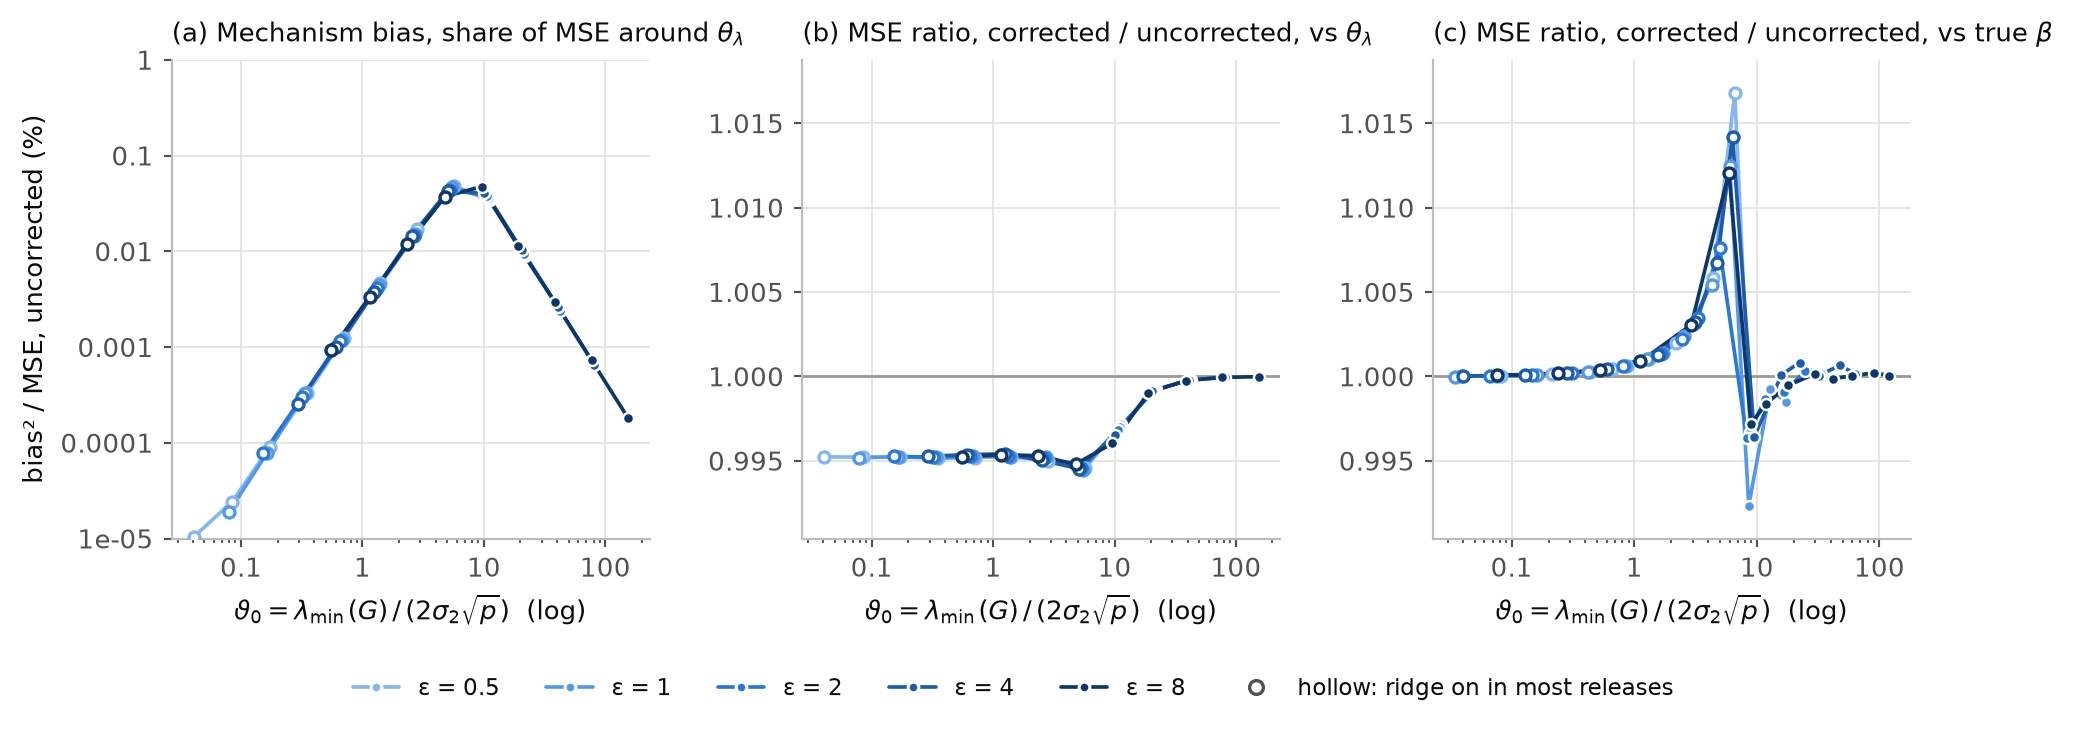
\includegraphics[width=\textwidth]{figures/bias_mse_ratio_v31.png}
  \caption{The optional correction under v3.1, $\delta = 10^{-9}$, $R^2 = 0.5$, against $\vartheta_0 = \lambda_{\min}(\bG)/(2\sigma_2\sqrt{p})$, one line per $\varepsilon$; hollow markers: the stage-1 ridge is on in most releases. (a)~Squared mechanism bias as a share of the mean squared error around $\btheta_\lambda$ (uncorrected estimate). (b)~Mean squared error of the corrected estimate divided by that of the uncorrected one, against $\btheta_\lambda$. (c)~The same against the true coefficients, from the cohort-level runs of Section~\ref{sec:eval:sim}. Values below 1 favour the correction.}
  \label{fig:bias_v31}
\end{figure}

% ---------------------------------------------------------------- 12.7
\subsection{Benchmark against AdaSSP}
\label{sec:eval:adassp}

AdaSSP~\cite{wang2018revisiting} perturbs the same sufficient statistics and solves a ridge whose penalty adapts to a private estimate of $\lambda_{\min}(\bX^{\top}\bX)$. It assumes one curator holding the joined table, which our setting rules out. The comparison therefore measures the utility cost of never pooling the data.

\paragraph{Setup.} We use the 29 UCI datasets~\cite{dua2019uci} of Wang's published evaluation, with 10-fold cross-validation on the folds of the earlier comparison. This subsection uses $\delta = 10^{-6}$, as Wang's published evaluation does. There are 50 noise draws per fold and $\varepsilon \in \{0.5, 1, 2, 4, 8\}$.
\begin{itemize}[noitemsep]
  \item \emph{Rows.} In each fold, $10\%$ of all rows, taken from the training folds, form a public reference set. Only the per-party preprocessing uses it, to fix its constants and bounds. Every arm trains on the remaining training rows ($80\%$ of the data) and is tested on the held-out fold.
  \item \emph{Split.} $\Rp$ holds the first $\lfloor d/2 \rfloor$ features and $\Op$ the rest and $y$. Every training row counts as matched.
\end{itemize}
We compare five arms.
\begin{itemize}[noitemsep]
  \item[(a)] \emph{AdaSSP (published):} Wang's algorithm and noise constants, with his preprocessing: z-scored features, each whole row scaled to unit norm, $y/\max|y|$. Its guarantee covers the whole record $(\bx, y)$.
  \item[(b)] \emph{AdaSSP (matched):} AdaSSP's adaptive ridge under our adjacency and our accountant. $\bA$ is exact; $\rho_{\mathrm{run}}/3$ goes to $\lambda_{\min}$ and $2\rho_{\mathrm{run}}/3$ to one joint release of the $\Op$-dependent entries with $\Delta = \sqrt{10}$, with the tight conversion. It is idealized, because its private $\lambda_{\min}$ step needs $\bX^{\top}\bX$ in the clear.
  \item[(c)] \emph{v3.1 with joint row normalization:} v3.1 on Wang's preprocessed data, without an intercept, with $B_R = B_O = B_y = 1$. It is idealized too. Wang's normalization scales each row $(\bx_R, \bx_O)$ by its joint norm, which needs both parties' features in one row, and no party has them in the vertical setting. The arm isolates the change of mechanism from the change of preprocessing.
  \item[(d)] \emph{v3.1 with block unit norm:} each party normalizes its own block of every row (Section~\ref{sec:protocol:preproc}), so $B_R^2 = 2$ with $\Rp$'s intercept and $B_O = 1$. $B_y$ is the $99.5\%$ quantile on the reference set.
  \item[(e)] \emph{v3.1 with standardization:} each party standardizes its own columns with reference-set constants; the bounds are the $99.5\%$ quantiles on the reference set.
\end{itemize}
The v3.1 arms run both releases, the stage-1 rule, the gate and the solve, with the bias correction off; a refused release would output $\btheta = 0$, but none was refused. Arms with different preprocessing have different non-private baselines. Each arm is therefore reported in two ways:
\begin{itemize}[noitemsep]
  \item as a ratio of its test MSE to that of its own non-private fit, $(\bZ^\top\bZ + \bI)^{-1}\bZ^\top\by$ (Wang's non-private estimator), on the same matched rows with the same preprocessing; arms (a)--(c) share this fit;
  \item as an absolute test MSE on one common scale, Wang's $y/\max|y|$, which adds the cost of the preprocessing.
\end{itemize}
Methods are compared by paired tests over folds (95\% CI of the mean difference of absolute test MSE, $t$ with 9 degrees of freedom).

\begin{table}[t]
  \centering
  \small
  \caption{Test MSE at $\varepsilon = 1$, $\delta = 10^{-6}$, as a ratio to each arm's own non-private fit. The first three columns give the non-private test MSE on Wang's $y/\max|y|$ scale under Wang's preprocessing (shared by (a)--(c)), block unit norm (d) and standardization (e). Last column: the earlier single-release mechanism from the previous version of this table (Wang's preprocessing, ratio to the same non-private fit as (a)--(c)).}
  \label{tab:adassp_v31}
  \setlength{\tabcolsep}{3.5pt}
  \begin{tabular}{@{}lrrrrrccccccc@{}}
    \toprule
    & & & \multicolumn{3}{c}{non-private test MSE} & \multicolumn{5}{c}{ratio to own non-private} & earlier \\
    \cmidrule(lr){4-6} \cmidrule(lr){7-11}
    Dataset & $n$ & $d$ & Wang & block & std. & (a) & (b) & (c) & (d) & (e) & VFL \\
    \midrule
    housing & 506 & 13 & 0.0400 & 0.0396 & 0.0320 & 1.83 & 2.03 & 2.46 & 2.50 & 3.25 & 1.97 \\
    wine & 1{,}599 & 11 & 0.0201 & 0.0252 & 0.0173 & 1.74 & 1.96 & 2.34 & 1.92 & 3.10 & 1.84 \\
    airfoil & 1{,}503 & 5 & 0.0534 & 0.0521 & 0.0504 & 1.10 & 1.16 & 1.47 & 1.51 & 1.86 & 1.16 \\
    concrete & 1{,}030 & 8 & 0.0445 & 0.0381 & 0.0490 & 1.54 & 1.74 & 2.35 & 2.69 & 2.41 & 1.69 \\
    bike & 17{,}379 & 17 & 0.0279 & 0.0270 & 0.0288 & 1.04 & 1.07 & 1.33 & 1.43 & 1.68 & 1.06 \\
    elevators & 16{,}599 & 18 & 0.00872 & 0.0229 & 0.00822 & 1.57 & 1.75 & 2.42 & 1.13 & 2.90 & 1.71 \\
    pol & 15{,}000 & 26 & 0.135 & 0.123 & 0.184 & 1.04 & 1.08 & 1.38 & 1.63 & 1.71 & 1.06 \\
    kin40k & 40{,}000 & 8 & 0.0632 & 0.0632 & 0.0634 & 1.00 & 1.00 & 1.00 & 1.00 & 1.00 & 1.00 \\
    protein & 45{,}730 & 9 & 0.119 & 0.121 & 0.119 & 1.01 & 1.01 & 1.04 & 1.03 & 1.15 & 1.01 \\
    \bottomrule
  \end{tabular}
\end{table}

\begin{table}[t]
  \centering
  \small
  \caption{Absolute test MSE at $\varepsilon = 1$, $\delta = 10^{-6}$, on Wang's $y/\max|y|$ scale; Table~\ref{tab:adassp_v31} gives the non-private test MSE on the same scale. Bold: lowest in the row.}
  \label{tab:adassp_abs_v31}
  \begin{tabular}{@{}lccccc@{}}
    \toprule
    & (a) AdaSSP, & (b) AdaSSP, & (c) v3.1, & (d) v3.1, & (e) v3.1, \\
    Dataset & published & matched & joint norm & block norm & standardize \\
    \midrule
    housing & \textbf{0.0732} & 0.0813 & 0.0982 & 0.0990 & 0.104 \\
    wine & \textbf{0.0350} & 0.0393 & 0.0469 & 0.0485 & 0.0537 \\
    airfoil & \textbf{0.0588} & 0.0620 & 0.0785 & 0.0787 & 0.0937 \\
    concrete & \textbf{0.0683} & 0.0774 & 0.105 & 0.103 & 0.118 \\
    bike & \textbf{0.0290} & 0.0299 & 0.0372 & 0.0388 & 0.0485 \\
    elevators & \textbf{0.0136} & 0.0153 & 0.0211 & 0.0260 & 0.0238 \\
    pol & \textbf{0.141} & 0.146 & 0.186 & 0.201 & 0.315 \\
    kin40k & 0.0633 & 0.0633 & 0.0633 & \textbf{0.0632} & 0.0634 \\
    protein & \textbf{0.120} & 0.120 & 0.124 & 0.124 & 0.137 \\
    \bottomrule
  \end{tabular}
\end{table}

\begin{table}[t]
  \centering
  \small
  \caption{Paired comparisons over all 29 datasets, $\delta = 10^{-6}$: number of datasets on which the first arm has significantly lower / higher absolute test MSE (95\% CI over folds). The remaining datasets show no significant difference.}
  \label{tab:verdicts_v31}
  \begin{tabular}{@{}lccccc@{}}
    \toprule
    Comparison & $\varepsilon = 0.5$ & $\varepsilon = 1$ & $\varepsilon = 2$ & $\varepsilon = 4$ & $\varepsilon = 8$ \\
    \midrule
    (d) v3.1, block vs (a) AdaSSP, published & 5 / 19 & 5 / 19 & 4 / 21 & 3 / 23 & 1 / 21 \\
    (c) v3.1, joint vs (a) AdaSSP, published & 7 / 19 & 6 / 20 & 3 / 22 & 2 / 22 & 0 / 23 \\
    (c) v3.1, joint vs (b) AdaSSP, matched & 10 / 17 & 8 / 18 & 5 / 20 & 5 / 21 & 3 / 20 \\
    (d) v3.1, block vs (c) v3.1, joint & 4 / 8 & 4 / 8 & 4 / 6 & 4 / 6 & 5 / 7 \\
    (e) v3.1, std.\ vs (d) v3.1, block & 1 / 25 & 2 / 25 & 2 / 25 & 2 / 24 & 2 / 23 \\
    \bottomrule
  \end{tabular}
\end{table}

\begin{figure}[t]
  \centering
  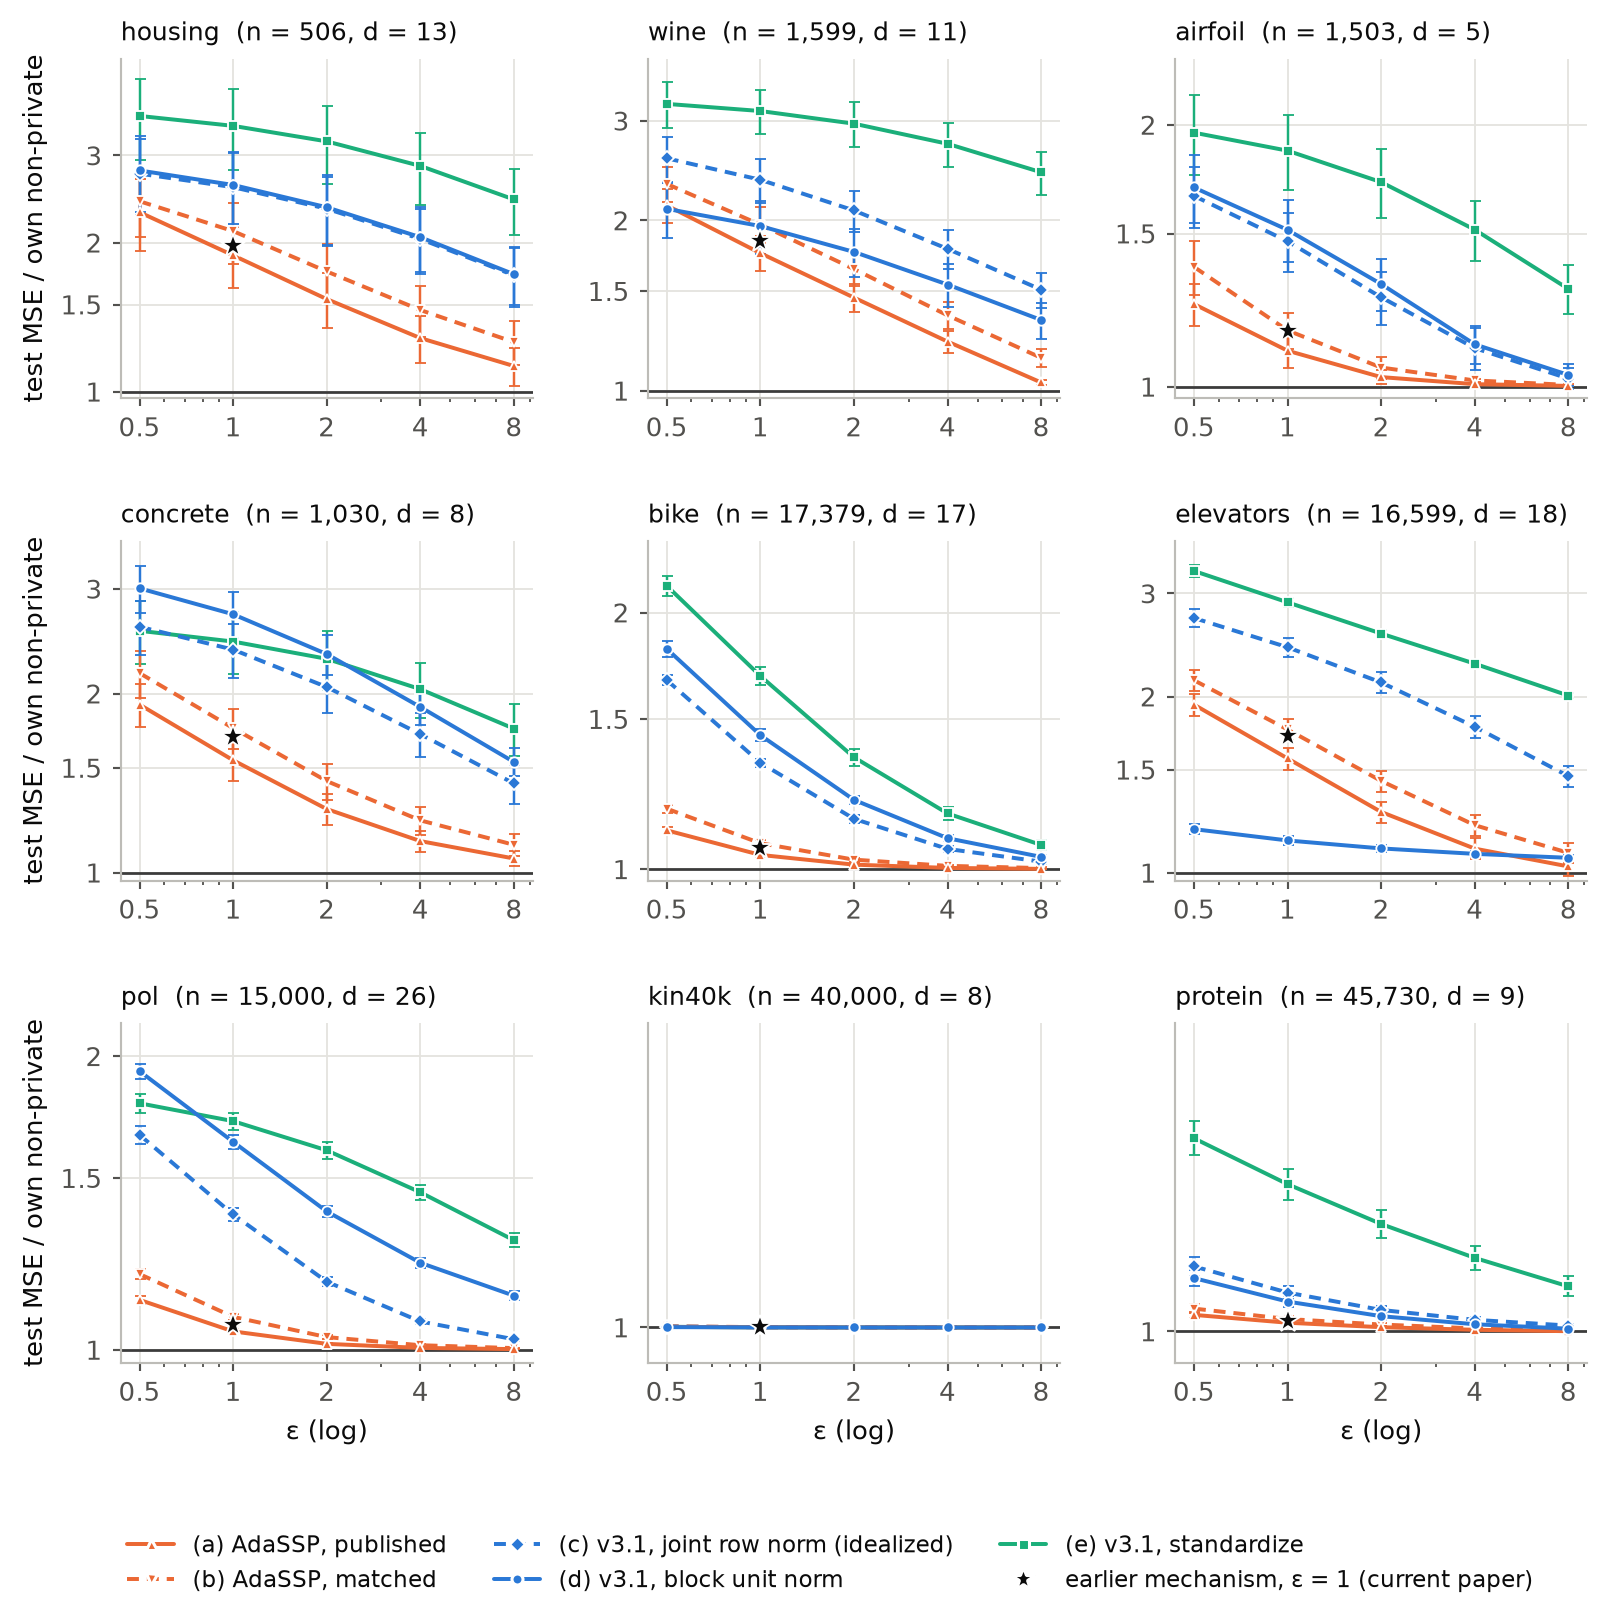
\includegraphics[width=\textwidth]{figures/adassp_mse_vs_eps_v31.png}
  \caption{Test MSE divided by each arm's own non-private test MSE against $\varepsilon$, $\delta = 10^{-6}$, on nine of the datasets. Points: mean over 10 folds and 50 noise draws. Error bars: 95\% CI of the mean ($t$ over folds). Stars: the earlier single-release mechanism at $\varepsilon = 1$, from the previous version of this comparison.}
  \label{fig:adassp_v31}
\end{figure}

\paragraph{Results.} Tables~\ref{tab:adassp_v31}--\ref{tab:verdicts_v31} and Figure~\ref{fig:adassp_v31} separate three effects.
\begin{itemize}
  \item \emph{The mechanism.} Arm (c) has the same preprocessing as AdaSSP. At $\varepsilon = 1$ it has significantly higher test MSE than AdaSSP (published) on 20 of 29 datasets and lower on 6, with a median gap of $+28\%$. Against AdaSSP (matched), which has our guarantee, it is higher on 18 and lower on 8, with a median gap of $+15\%$. The earlier mechanism beat AdaSSP (matched) on 27 of 29 datasets at $\varepsilon \le 1$. v3.1 is significantly worse than AdaSSP (matched) on 17--21 datasets, and better on 3--10, at every $\varepsilon$ from $0.5$ to $8$.

  The cause is the ridge, not the noise. For unit bounds at $\varepsilon = 1$, the stage-2 noise of v3.1 ($\sigma_2 = 15.1$) is lower than that of AdaSSP (matched) ($17.6$). But the stage-1 rule sets $\lambda \approx g^\star + r_1 - \lambda_{\min}(\hat\bG_1)$, which certifies $\vartheta \ge \vartheta^\star = 2.5$ with probability $1 - \alpha_L$ from a release that has only $10\%$ of the budget. Its median ridge at $\varepsilon = 1$ is $3.2$--$5.8$ times that of AdaSSP (matched) and $4.7$--$12$ times that of AdaSSP (published), for example $786$, $188$ and $127$ on housing and $559$, $150$ and $101$ on protein. The earlier mechanism's fixed ridge $2\vartheta^\star\sigma\sqrt p$ with $\vartheta^\star = 2$ was $193$ on housing.

  v3.1 is ahead only where there is little linear signal (forest, fertility, pendulum, pumadyn32nm, solar, tamielectric), and there shrinking towards zero costs little. On the largest datasets (3droad, kin40k, tamielectric) all arms are within $0.1\%$ of non-private.
  \item \emph{The preprocessing.} Block normalization (d) and joint normalization (c) differ significantly on only 12 of 29 datasets in absolute test MSE ($\varepsilon = 1$), and their ratios to their own non-private fits are similar. Their differences come from the non-private fits: on elevators, block normalization's non-private test MSE is $2.6$ times that of Wang's preprocessing, while on concrete it is $0.86$ times. Plain standardization (e) is worse than block normalization on 23--25 datasets, because heavy tails inflate the bounds.
  \item \emph{The implementable protocol.} Arm (d) has higher test MSE than AdaSSP (published) on 19 of 29 datasets at $\varepsilon = 1$ and lower on 5. The median gap is $+31\%$ at $\varepsilon = 1$ and $+12\%$ at $\varepsilon = 8$. On protein the gap is $3.6\%$ ($0.124$ against $0.120$), and on bike it is $34\%$.
\end{itemize}

\paragraph{AdaSSP's published noise constants.} AdaSSP adds noise of s.d.\ $s = \sqrt{\log(6/\delta)}/(\varepsilon/3)$ to each of three statistics: $\lambda_{\min}$, $\bX^\top\bX$ (symmetrized, so off-diagonal s.d.\ $s/\sqrt2$) and $\bX^\top\by$.
\begin{itemize}[noitemsep]
  \item Under add/remove adjacency each of the three has sensitivity $1$ for unit-norm rows. The three releases then cost $\rho = 3/(2s^2)$, which the tight conversion turns into $(0.31, 0.64, 1.35, 2.87, 6.24)$-DP at $\delta = 10^{-6}$ for nominal $\varepsilon = (0.5, 1, 2, 4, 8)$, which is valid, with room.
  \item Under replace-one adjacency, which is ours, the sensitivities of $\bX^\top\bX$ (the Frobenius norm of $\bx\bx^\top - \bx'\bx'^\top$, which matches the symmetrized noise) and of $\bX^\top\by$ are $\sqrt2$ and $2$. The same constants then give $(0.48, 1.01, 2.14, 4.60, 10.2)$-DP.
  \item Recalibrated to exactly $(\varepsilon, \delta)$ under replace-one adjacency, with the tight conversion and an equal split, AdaSSP's test MSE rises by a median $2$--$3\%$ (range $-5\%$ to $+28\%$).
\end{itemize}
The published column therefore overstates AdaSSP's advantage only slightly. The gap to v3.1 lies in the ridge rule.

\tocheck{AdaSSP's adjacency: the published constants are consistent with add/remove adjacency (sensitivity 1 for each statistic); confirm against the statement in Wang (2018) before citing it.}

\tocheck{The v3.1 ridge is sized for interval validity (theta-star = 2.5, r-1 at the 1 - alpha-L quantile from 10 percent of the budget), not for prediction. The levers of Section 9.5 (exact-quantile r-1, f-1 near 0.35) would shrink it by about 37 percent; rerun this comparison with them if they become the evaluation's settings.}

% ---------------------------------------------------------------- 12.8
\subsection{Intersection size on real data}
\label{sec:eval:sweep}

Figure~\ref{fig:sweep_v31} repeats the experiment of Figure~\ref{fig:sim_rmse_v31} on the four datasets with at least 15{,}000 rows and a real linear signal: bike, elevators, pol and protein. The settings are those of Section~\ref{sec:eval:sim}, with $\delta = 10^{-9}$ for v3.1 and for AdaSSP alike.
\begin{itemize}[noitemsep]
  \item In each fold the reference set is set aside as in Section~\ref{sec:eval:adassp}. The remaining training rows are shuffled once, and the first $n$ form the matched set, nested across $n$. The held-out fold is the test set.
  \item There are 40 noise draws per fold and $n$.
  \item Each arm is compared with its own non-private fit at the same $n$.
\end{itemize}
Table~\ref{tab:sweep_v31} gives the $n$ at which v3.1 with block normalization, and AdaSSP (published), come within $10\%$ of non-private test MSE.

\begin{figure}[t]
  \centering
  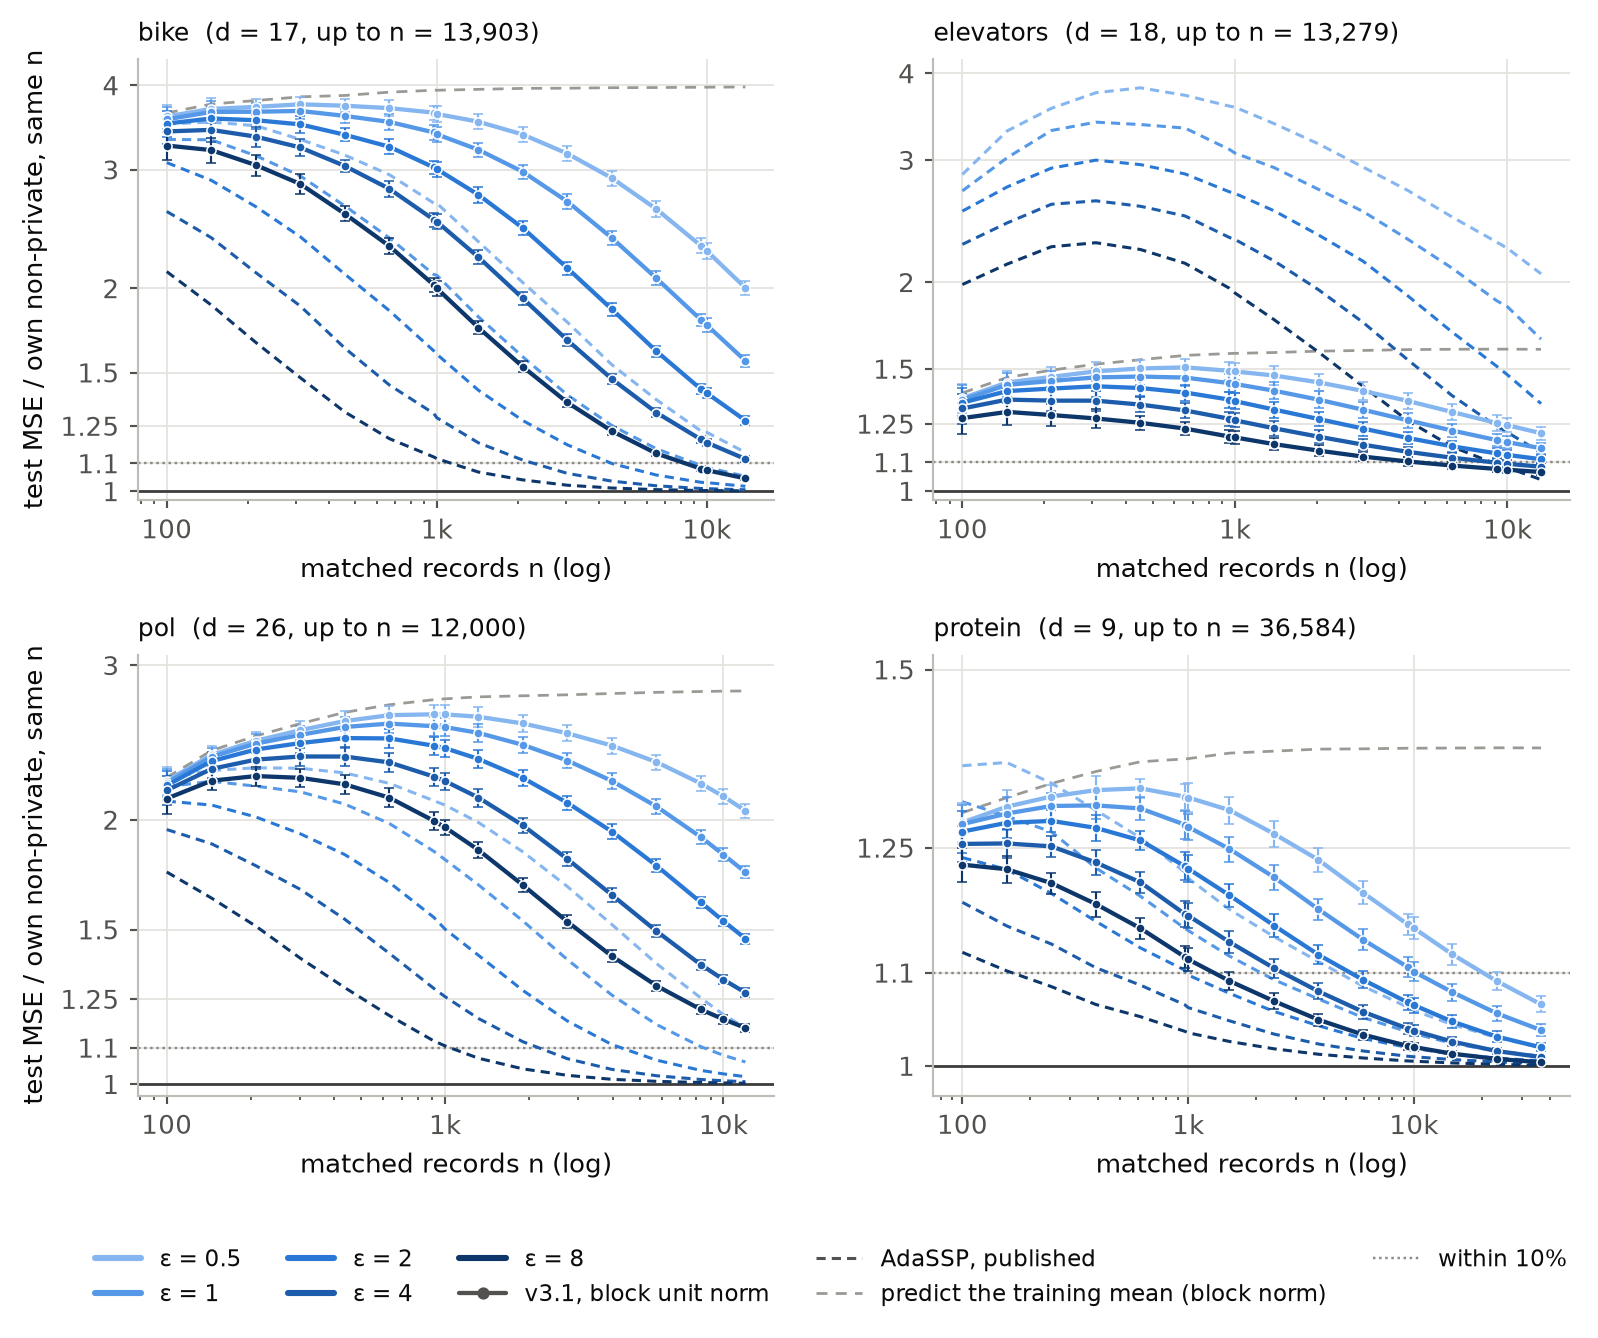
\includegraphics[width=\textwidth]{figures/sweep_n_v31.png}
  \caption{Test MSE divided by the arm's own non-private test MSE at the same $n$, against the number of matched records, $\delta = 10^{-9}$. Solid: v3.1 with block unit norm. Dashed: AdaSSP (published). Colour: $\varepsilon$. Error bars: 95\% CI over folds.}
  \label{fig:sweep_v31}
\end{figure}

\begin{table}[t]
  \centering
  \small
  \caption{Matched records needed to come within $10\%$ of the arm's own non-private test MSE, $\delta = 10^{-9}$: v3.1 with block unit norm, with AdaSSP (published) in brackets. ``$>$'' means not reached at the sizes available.}
  \label{tab:sweep_v31}
  \setlength{\tabcolsep}{4.5pt}
  \begin{tabular}{@{}lrccccc@{}}
    \toprule
    Dataset & $n$ available & $\varepsilon = 0.5$ & $\varepsilon = 1$ & $\varepsilon = 2$ & $\varepsilon = 4$ & $\varepsilon = 8$ \\
    \midrule
    bike & 13{,}903 & $>$14k ($>$14k) & $>$14k (9.1k) & $>$14k (4.4k) & $>$14k (2.3k) & 8.3k (1.1k) \\
    elevators & 13{,}279 & $>$13k ($>$13k) & $>$13k ($>$13k) & $>$13k ($>$13k) & 8.9k ($>$13k) & 4.7k (8.7k) \\
    pol & 12{,}000 & $>$12k ($>$12k) & $>$12k (8.5k) & $>$12k (4.3k) & $>$12k (2.2k) & $>$12k (1.0k) \\
    protein & 36{,}584 & 20k (4.6k) & 10k (2.1k) & 5.2k (1.0k) & 2.6k (0.4k) & 1.3k (0.2k) \\
    \bottomrule
  \end{tabular}
\end{table}

\begin{itemize}
  \item \emph{Protein.} v3.1 comes within $10\%$ of non-private at $20$k, $10$k, $5.2$k, $2.6$k and $1.3$k matched records for $\varepsilon = 0.5$ to $8$; doubling $\varepsilon$ halves the records needed. The earlier mechanism needed $5.4$k, $2.8$k, $1.4$k and $619$ for $\varepsilon = 0.5$ to $4$. AdaSSP needs $4.4$--$7.8$ times fewer records than v3.1, against $1.4$--$2.1$ times fewer than the earlier mechanism.
  \item \emph{Bike and pol.} v3.1 gets within $10\%$ only on bike at $\varepsilon = 8$ ($8.3$k). At the largest size available its test MSE is $1.56$ and $1.74$ times non-private at $\varepsilon = 1$, and $1.12$ and $1.27$ times at $\varepsilon = 4$.
  \item \emph{Elevators.} The entries for v3.1 are relative to block normalization's own non-private fit, which is $2.8$ times worse than that on standardized features. Against the standardized non-private fit, v3.1 with block normalization never comes within $10\%$ at these sizes.
  \item \emph{The ridge stays on throughout.} At the largest $n$ and $\varepsilon = 1$ the median stage-1 ridge is $1{,}334$ on protein and $2{,}226$ on bike. Section~\ref{sec:stats:noff} puts the switch-off for protein at $691$k matched records at $\varepsilon = 1$.
\end{itemize}
% ---------------------------------------------------------------- END-SECTIONS
